\section{Experiments}
\label{sec:exp}

The pre-registered experiments answer RQ1 to RQ3 in turn, and the planned exploratory ones RQ4;
Table~\ref{tab:tests} gathers every confirmatory test. All analyses use Python with
MNE~\cite{gramfort2013}, pyRiemann~\cite{pyriemann}, scikit-learn~\cite{pedregosa2011},
braindecode~\cite{braindecode} and PyTorch~\cite{paszke2019}, with the healthy datasets from
MOABB~\cite{jayaram2018moabb}. Classical methods ran on an \demoInferenceMachine{} laptop and
every EEGNet of the main study on a \dlPretrainDevice{} GPU in Kaggle notebooks (pre-training the
\dlPretrainModels{} models took \dlPretrainMinutes{} GPU minutes).

\subsection{RQ1: leakage in the published protocol (H1, H1b)}
\label{sec:leak}
The published protocol inflated accuracy for every patient. Rebuilt as the dataset's script does
it, the authors' recipe scored \rqOneCspLdaReplicaPaperReplicaMean\,\% on hand against sixth
finger, where the dataset paper gives
\rqOnePublishedGroupBCspLda--\rqOnePublishedGroupTCspLda\,\%~\cite{wang2026dataset}, and
\rqOneCspLdaReplicaCvLeakfreeMean\,\% under leakage-free cross-validation; we reproduce the
direction of the leak, not the published number. For the pre-registered test our own CSP+LDA
pipeline reached \rqOneCspLdaPaperReplicaMean\,\% (95\,\% CI
\rqOneCspLdaPaperReplicaCiLo--\rqOneCspLdaPaperReplicaCiHi) when the filters saw all trials and
\rqOneCspLdaCvLeakfreeMean\,\% (\rqOneCspLdaCvLeakfreeCiLo--\rqOneCspLdaCvLeakfreeCiHi) when every
step stayed inside the training folds (Fig.~\ref{fig:leak}). The inflation averaged
\rqOneHOneDiff{} points (CI \rqOneHOneDiffCiLo--\rqOneHOneDiffCiHi; per patient
\rqOneHOneDiffMin{} to \rqOneHOneDiffMax; $W = \rqOneHOneW$, $p = \rqOneHOneP$,
$r = \rqOneHOneR$, $n = \rqOneHOneN$): H1 is \rqOneHOneCategory. With so little signal even the
leakage-free estimate fell below chance for \rqOneCspLdaCvLeakfreeNBelowChance{} of
\rqOneHOneN{} patients (lowest \rqOneCspLdaCvLeakfreeMin\,\%), and MDM averaged
\rqOneMdmCvLeakfreeMean\,\%. Against the splits that keep whole runs apart, the leaky score was
higher by \rqOneCspLdaPaperReplicaMinusLoroDiff{} points than leave one run out (CI
\rqOneCspLdaPaperReplicaMinusLoroDiffCiLo--\rqOneCspLdaPaperReplicaMinusLoroDiffCiHi) and by
\rqOneCspLdaPaperReplicaMinusChronoDiff{} points than the chronological split
(\rqOneCspLdaPaperReplicaMinusChronoDiffCiLo--\rqOneCspLdaPaperReplicaMinusChronoDiffCiHi), both
descriptive. TS+LR and MDM, which fit nothing with labels before the classifier, were unaffected
(\rqOneTsLrLeakDiff{} and \rqOneMdmLeakDiff{} points). On healthy volunteers the same code added
\rqOneBnciHOneBDiff{} points on BNCI2014\_001 ($n = \rqOneBnciHOneBN$) and \rqOneChoHOneBDiff{} on
Cho2017 ($n = \rqOneChoHOneBN$), so H1b is supported: the leak lies in the procedure, not in
these recordings. Measured without it, five classical methods (CSP with LDA or SVM, filter-bank CSP with LDA,
TS+LR and MDM, under either run-wise split) reached only
\rqOneHeldOutRunsMeanMin--\rqOneHeldOutRunsMeanMax\,\% on hand against sixth finger, against
\rqOneSfRestHeldOutRunsMeanMin--\rqOneSfRestHeldOutRunsMeanMax\,\% on sixth finger against
rest: the two movements barely separate, while movement and rest do.

\begin{figure}[!t]
  \centering
  \begin{minipage}[t]{0.485\textwidth}
  \vspace{0pt}\centering
  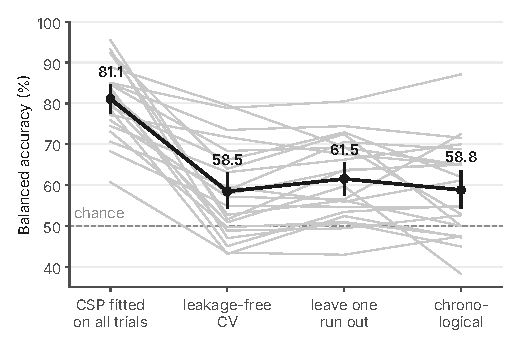
\includegraphics{paper_leak.pdf}
  \caption{Accuracy drops for nearly every patient once test trials no longer shape the CSP
  filters.
  Hand against sixth finger, CSP+LDA, pre-therapy session ($n = \rqOneN$), under the four
  protocols of Fig.~\ref{fig:protocols}. Grey: one line per patient; black: mean and 95\,\%
  bootstrap CI; dashed: chance.}
  \label{fig:leak}
  \end{minipage}\hfill
  \begin{minipage}[t]{0.485\textwidth}
  \vspace{0pt}\centering
  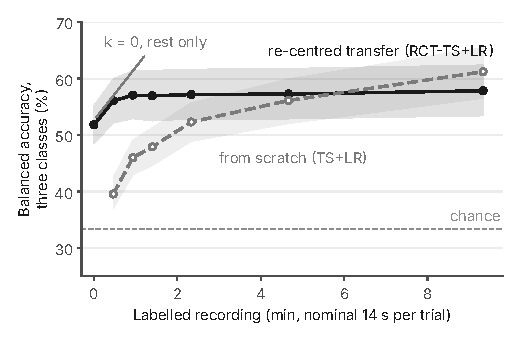
\includegraphics{paper_calibration.pdf}
  \caption{Transfer starts a new patient high and then stays almost flat. Three classes,
  pre-therapy session ($n = \rqTwoHTwoAN$). Solid: RCT-TS+LR, transfer at target weight
  \rqTwoHparamRctTslrWeight; dashed: TS+LR on the patient alone. Points at the nominal minutes
  of labelled recording for $k = 0$ (re-centred on \rqTwoRestMinutes\,min of unlabelled rest,
  drawn at 0), 1, 2, 3, 5, 10 and all trials; bands: 95\,\%
  bootstrap CIs. The final gap was not tested.}
  \label{fig:setup}
  \end{minipage}
\end{figure}

\subsection{RQ2: calibration for a new patient (H2a, H2b)}
\label{sec:newuser}
Re-centred transfer gave a new patient a fast start and then hardly changed (Fig.~\ref{fig:setup}).
After one trial of each movement it scored \rqTwoRestAhSfRctTslrKOneMean\,\% on three classes (CI
\rqTwoRestAhSfRctTslrKOneCiLo--\rqTwoRestAhSfRctTslrKOneCiHi), and \rqTwoRestAhSfRctTslrKZeroMean\,\%
with no labelled trial at all. Without transfer, TS+LR learned
\rqTwoRestAhSfTsLrKOneMean\,\% (\rqTwoRestAhSfTsLrKOneCiLo--\rqTwoRestAhSfTsLrKOneCiHi) from the
four windows of $k = 1$, \rqTwoRestAhSfTsLrKFiveMean\,\% at $k = 5$, and needed $k = 10$ to reach
\rqTwoRestAhSfTsLrKTenMean\,\%, the level transfer offered after one trial. Transfer held near its
start, \rqTwoRestAhSfRctTslrKFiveMean\,\% at $k = 5$ and \rqTwoRestAhSfRctTslrKAllMean\,\% with
every trial, while the patient-only decoder reached \rqTwoRestAhSfTsLrKAllMean\,\%. We did not
test this final gap of \rqTwoRestAhSfTsLrMinusRctTslrKAllDiff{} points
(\rqTwoRestAhSfTsLrMinusRctTslrKAllDiffCiLo{} to \rqTwoRestAhSfTsLrMinusRctTslrKAllDiffCiHi;
\rqTwoRestAhSfTsLrMinusRctTslrKAllBetter{} patients better off without transfer,
\rqTwoRestAhSfTsLrMinusRctTslrKAllWorse{} with it).

Both confirmatory tests point the same way (Table~\ref{tab:tests}). Transfer had the larger ALC
(mean difference \rqTwoHTwoADiff, CI \rqTwoHTwoADiffCiLo--\rqTwoHTwoADiffCiHi, median
\rqTwoHTwoAMedianDiff, $W = \rqTwoHTwoAW$, $p = \rqTwoHTwoAP$, $r = \rqTwoHTwoAR$), so H2a is
supported, though much of this comes from budgets at which the patient-only decoder has almost
nothing to learn from: transfer without a labelled trial, re-centred on
\rqTwoRestMinutes\,min of unlabelled rest, already matched it at $k = 5$. The lead
at $k = 5$ was \rqTwoHTwoBPointsDiff{} points larger than with the whole pool
($p = \rqTwoHTwoBP$), which supports H2b. Per budget (secondary, Holm-adjusted) transfer led by
\rqTwoAdvantageKOneDiff{} points at $k = 1$ ($p = \rqTwoAdvantageKOnePHolm$),
\rqTwoAdvantageKFiveDiff{} at $k = 5$ ($p = \rqTwoAdvantageKFivePHolm$) and
\rqTwoAdvantageKTenDiff{} at $k = 10$ ($p = \rqTwoAdvantageKTenPHolm$). Both tests held without
the development patients, under the chronological draw and after therapy. Of the
\rqTwoHTwoAN{} patients, \rqTwoReachRestAhSfSixtyBoth{} reached 60\,\% with both methods,
transfer getting there a median of \rqTwoReachRestAhSfSixtyMedianSaved{} trials per movement
earlier; \rqTwoReachRestAhSfSixtyOnlyScratch{} got there only without transfer,
\rqTwoReachRestAhSfSixtyOnlyTransfer{} only with it and \rqTwoReachRestAhSfSixtyNeither{} not at
all (for 70\,\%: \rqTwoReachRestAhSfSeventyBoth, \rqTwoReachRestAhSfSeventyOnlyScratch,
\rqTwoReachRestAhSfSeventyOnlyTransfer{} and \rqTwoReachRestAhSfSeventyNeither). The secondary
EEGNet pair supported H2a and H2b too: pre-trained, the network gave
\rqTwoRestAhSfEegnetEaFtKZeroMean\,\% before any labelled trial and
\rqTwoRestAhSfEegnetEaFtKAllMean\,\% with all of them, while the network trained on the patient
alone rose from \rqTwoRestAhSfEegnetScratchKOneMean\,\% to \rqTwoRestAhSfEegnetScratchKAllMean\,\%.

\begin{table*}[!t]
  \centering
  \caption{Results of the pre-registered tests on the pre-therapy session. Each effect is the
  mean paired difference with its 95\,\% bootstrap CI: in points of balanced accuracy, apart
  from H2a and H3, which use the ALC scale (0 for chance, 1 for a perfect decoder). Tests of
  H1, H1b, H2b and H3c are one-sided, those of H2a and H3 two-sided. $W$ is the sum of positive
  ranks (one-sided) or the smaller rank sum (two-sided); $^\dagger$ marks $p$-values
  Holm-adjusted within a family of two. Unless a row says otherwise, the comparison is transfer
  minus no transfer, over $n = \rqTwoHTwoAN$ patients. The final column gives the category when
  the test is repeated after therapy ($n = \nPost$; unchanged when sub-21 and sub-22 are
  averaged, $n = \rqOneHOnePostLinkedN$).}
  \label{tab:tests}
  \footnotesize
  \setlength{\tabcolsep}{2.4pt}
  \begin{tabular}{@{}llccccll@{}}
    \toprule
    & Comparison, per patient & Mean diff.\ [95\,\% CI] & $W$ & $r$ & $p$ & Outcome & After therapy \\
    \midrule
    H1 & CSP+LDA, hand vs finger: leaky $-$ leakage-free & \rqOneHOneDiff{} [\rqOneHOneDiffCiLo, \rqOneHOneDiffCiHi] & \rqOneHOneW & \rqOneHOneR & \rqOneHOneP & \rqOneHOneCategory & \rqOneHOnePostCategory \\
    H1b & The same, BNCI2014\_001, healthy ($n = \rqOneBnciHOneBN$) & \rqOneBnciHOneBDiff{} [\rqOneBnciHOneBDiffCiLo, \rqOneBnciHOneBDiffCiHi] & \rqOneBnciHOneBW & \rqOneBnciHOneBR & \rqOneBnciHOneBPHolm$^\dagger$ & supported & -- \\
     & The same, Cho2017, healthy ($n = \rqOneChoHOneBN$) & \rqOneChoHOneBDiff{} [\rqOneChoHOneBDiffCiLo, \rqOneChoHOneBDiffCiHi] & \rqOneChoHOneBW & \rqOneChoHOneBR & \rqOneChoHOneBPHolm$^\dagger$ & supported & -- \\
    H2a & New user, three classes, ALC & \rqTwoHTwoADiff{} [\rqTwoHTwoADiffCiLo, \rqTwoHTwoADiffCiHi] & \rqTwoHTwoAW & \rqTwoHTwoAR & \rqTwoHTwoAP & \rqTwoHTwoACategory & \rqTwoHTwoAPostCategory \\
    H2b & New user: lead at $k = 5$ $-$ lead with all & \rqTwoHTwoBPointsDiff{} [\rqTwoHTwoBPointsDiffCiLo, \rqTwoHTwoBPointsDiffCiHi] & \rqTwoHTwoBW & \rqTwoHTwoBR & \rqTwoHTwoBP & \rqTwoHTwoBCategory & \rqTwoHTwoBPostCategory \\
    H3 (a) & New command, finger vs rest, ALC & \rqThreeHThreeADiff{} [\rqThreeHThreeADiffCiLo, \rqThreeHThreeADiffCiHi] & \rqThreeHThreeAW & \rqThreeHThreeAR & \rqThreeHThreeAPHolm$^\dagger$ & \rqThreeHThreeACategory & \rqThreeHThreeAPostCategory \\
    H3 (b) & New command, three classes, ALC & \rqThreeHThreeBDiff{} [\rqThreeHThreeBDiffCiLo, \rqThreeHThreeBDiffCiHi] & \rqThreeHThreeBW & \rqThreeHThreeBR & \rqThreeHThreeBPHolm$^\dagger$ & \rqThreeHThreeBCategory & \rqThreeHThreeBPostCategory \\
    H3c & Finger vs rest, $k = 2$: $-$ own-hand decoder & \rqThreeHThreeCKTwoPointsDiff{} [\rqThreeHThreeCKTwoPointsDiffCiLo, \rqThreeHThreeCKTwoPointsDiffCiHi] & \rqThreeHThreeCKTwoW & \rqThreeHThreeCKTwoR & \rqThreeHThreeCKTwoPHolm$^\dagger$ & \rqThreeHThreeCKTwoCategory & \rqThreeHThreeCKTwoPostCategory \\
     & The same, $k = 5$ & \rqThreeHThreeCKFivePointsDiff{} [\rqThreeHThreeCKFivePointsDiffCiLo, \rqThreeHThreeCKFivePointsDiffCiHi] & \rqThreeHThreeCKFiveW & \rqThreeHThreeCKFiveR & \rqThreeHThreeCKFivePHolm$^\dagger$ & \rqThreeHThreeCKFiveCategory & \rqThreeHThreeCKFivePostCategory \\
    \midrule
    \multicolumn{8}{@{}l}{\emph{Secondary pair: EEGNet pre-trained and fine-tuned $-$ EEGNet from scratch}} \\
    H2a & New user, three classes, ALC & \rqTwoEegnetHTwoADiff{} [\rqTwoEegnetHTwoADiffCiLo, \rqTwoEegnetHTwoADiffCiHi] & \rqTwoEegnetHTwoAW & \rqTwoEegnetHTwoAR & \rqTwoEegnetHTwoAP & \rqTwoEegnetHTwoACategory & -- \\
    H2b & New user: lead at $k = 5$ $-$ lead with all & \rqTwoEegnetHTwoBPointsDiff{} [\rqTwoEegnetHTwoBPointsDiffCiLo, \rqTwoEegnetHTwoBPointsDiffCiHi] & \rqTwoEegnetHTwoBW & \rqTwoEegnetHTwoBR & \rqTwoEegnetHTwoBP & \rqTwoEegnetHTwoBCategory & -- \\
    H3 (a) & New command, finger vs rest, ALC & \rqThreeEegnetHThreeADiff{} [\rqThreeEegnetHThreeADiffCiLo, \rqThreeEegnetHThreeADiffCiHi] & \rqThreeEegnetHThreeAW & \rqThreeEegnetHThreeAR & \rqThreeEegnetHThreeAPHolm$^\dagger$ & \rqThreeEegnetHThreeACategory & -- \\
    H3 (b) & New command, three classes, ALC & \rqThreeEegnetHThreeBDiff{} [\rqThreeEegnetHThreeBDiffCiLo, \rqThreeEegnetHThreeBDiffCiHi] & \rqThreeEegnetHThreeBW & \rqThreeEegnetHThreeBR & \rqThreeEegnetHThreeBPHolm$^\dagger$ & \rqThreeEegnetHThreeBCategory & -- \\
    \bottomrule
  \end{tabular}
\end{table*}

\subsection{RQ3: a new command (H3, H3c)}
\label{sec:newcommand}
Before therapy the confirmatory pair found no clear gain from transfer for the new command
(Fig.~\ref{fig:rqthree}). Outcome (a), sixth finger against rest, uses no hand trial
(Fig.~\ref{fig:calib}c) and so traces how a command is learned from nothing: with one
sixth-finger trial transfer scored \rqThreeSfRestRctTslrKOneMean\,\% and the patient-only decoder
\rqThreeSfRestTsLrKOneMean\,\%, with five \rqThreeSfRestRctTslrKFiveMean\,\% and
\rqThreeSfRestTsLrKFiveMean\,\%. The ALC difference leaned towards transfer, but its CI crossed
zero (median \rqThreeHThreeAMedianDiff, Holm $p = \rqThreeHThreeAPHolm$). Outcome (b), three
classes, does use the hand trials. There the patient-only decoder, fitted on unbalanced classes
without class weights as the plan required, hardly ever said ``sixth finger'' (recall
\rqThreeRestAhSfTsLrSfRecallMin--\rqThreeRestAhSfTsLrSfRecallMax\,\% for $k \leq 5$), whereas
transfer recalled \rqThreeRestAhSfRctTslrKFiveSfRecall\,\% at $k = 5$; still the ALC gap was small
(median \rqThreeHThreeBMedianDiff, $p = \rqThreeHThreeBPHolm$). H3 is thus inconclusive. After
therapy outcome (a) reached significance (Holm $p = \rqThreeHThreeAPostPHolm$), so H3 was
supported in that session and did not replicate. The secondary EEGNet pair preferred transfer on
both outcomes (finger against rest: ALC difference \rqThreeEegnetHThreeADiff, CI
\rqThreeEegnetHThreeADiffCiLo--\rqThreeEegnetHThreeADiffCiHi, Holm
$p = \rqThreeEegnetHThreeAPHolm$), but a network trained on the patient alone is weak at these
budgets (\rqThreeSfRestEegnetScratchKOneMean\,\% on finger against rest after one trial), so this
says more about EEGNet than about the new command.

The planned own-hand control asks whether the sixth finger adds anything a hand decoder lacks.
Never shown a sixth-finger trial, it detected sixth-finger windows at
\rqThreeSfRestAhProxyMean\,\% (CI \rqThreeSfRestAhProxyCiLo--\rqThreeSfRestAhProxyCiHi), above
transfer at $k = 2$ (\rqThreeSfRestRctTslrKTwoMean\,\%) and $k = 5$
(\rqThreeSfRestRctTslrKFiveMean\,\%). Both one-sided tests failed (Holm
$p = \rqThreeHThreeCKTwoPHolm$ each) with CIs entirely below zero, so H3c is inconclusive and the
hand decoder came out ahead. These detectors also flagged most hand-imagery windows as ``sixth
finger'' (own-hand decoder \rqThreeHandAsFingerAhProxy\,\%, transfer
\rqThreeHandAsFingerRctTslrKAll--\rqThreeHandAsFingerRctTslrKOne\,\% for $k \geq 1$). Following
the plan we claim no separate sixth-finger command: what is detected may be imagined movement of
any kind.

\begin{figure}[!t]
  \centering
  \begin{minipage}[t]{0.485\textwidth}
  \vspace{0pt}\centering
  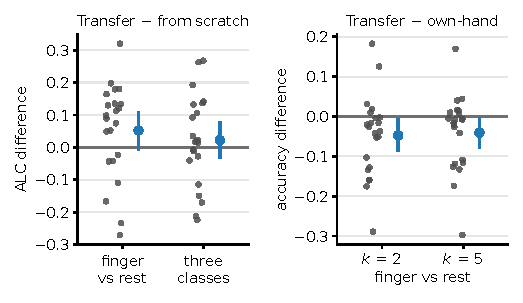
\includegraphics{rq3_patients.pdf}
  \caption{For the new command transfer gave no clear gain, and a decoder that never saw a
  sixth-finger trial scored higher. Pre-therapy session ($n = \rqThreeHThreeAN$), one grey point per
  patient. Left: ALC over $k = 1, 2, 3, 5$, RCT-TS+LR minus TS+LR, for finger against rest (H3a)
  and three classes (H3b). Right: RCT-TS+LR minus the own-hand decoder on finger against rest,
  in points (H3c). Black: mean and 95\,\% CI; positive values favour transfer.}
  \label{fig:rqthree}
  \end{minipage}\hfill
  \begin{minipage}[t]{0.485\textwidth}
  \vspace{0pt}\centering
  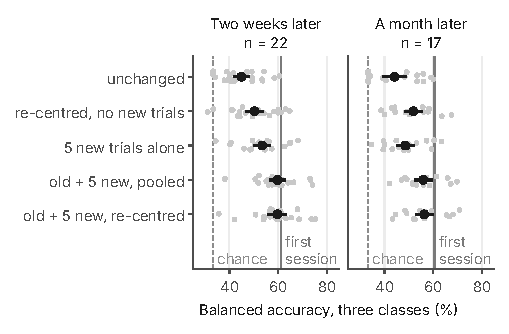
\includegraphics{paper_later.pdf}
  \caption{A decoder does not carry over to another day, but a few new trials win most of it
  back. Exploratory; three classes, runs 3--4. The first session's TS+LR decoder used as it is,
  re-centred on the new day's rest, replaced by one trained on five new trials per movement, or
  retrained on the old session plus five new trials, pooled or re-centred. Grey: patients;
  black: mean and 95\,\% CI; solid grey line: the same method within the first session; dashed:
  chance.}
  \label{fig:later}
  \end{minipage}
\end{figure}

\subsection{RQ4: continuous replay and later days (exploratory)}
\label{sec:later}
\emph{Continuous replay (H4, pre-registered).} H4's prediction failed. With runs 3--4 streamed
as one signal (a 4\,s window every 0.5\,s) through the gate as fixed before any replay, the
three-class decoders trained on the whole pool (CSP+LDA, TS+LR, RCT-TS+LR and EEGNet without
transfer) produced the sixth-finger command in only
\rqFourReplayFingerDetectMin--\rqFourReplayFingerDetectMax\,\% of sixth-finger periods, made
\rqFourReplayFalsePerMinMin--\rqFourReplayFalsePerMinMax{} false activations per minute of rest,
and transferred \rqFourReplayItrMin--\rqFourReplayItrMax{} bit/min, about the same as the
\rqFourReplaySilentItr{} bit/min that this measure credits to a gate that never fires.

\emph{Other days.} Decoders did not survive the move to a later session (Fig.~\ref{fig:later}).
TS+LR trained on the first session scored \rqFourLaterPostWithinPreMean\,\% within it,
\rqFourLaterPostUnchangedMean\,\% two weeks later ($n = \rqFourLaterPostUnchangedN$), alike after
BCI training (\rqFourLaterPostUnchangedGroupBMean\,\%) and conventional therapy
(\rqFourLaterPostUnchangedGroupTMean\,\%), and \rqFourLaterFollowUnchangedMean\,\% a month on
($n = \rqFourLaterFollowUnchangedN$). Re-centring on the new day's rest, which needs no labels,
won back part of the loss (\rqFourLaterPostRecentredKZeroMean\,\% and
\rqFourLaterFollowRecentredKZeroMean\,\%), and five new trials per movement added to the old
session won back more. Across the four questions, then, the leak is large, transfer helps only at
the start, and nothing yet separates the sixth finger from the hand.
